\documentclass{article}
\usepackage{blindtext}
\usepackage[a4paper, total={6in, 8in}]{geometry}
\usepackage{float} % here for H placement parameter
\usepackage{graphicx}
\graphicspath{ {./images/} }

\title{Quantitative Cell and Tissue Analysis}
\author{Lucas Comyn}

\begin{document}
\maketitle


\section{Block I}
 \subsection{Abbreviations}
\begin{table}[H]
\centering
\begin{tabular}{|l|l|}
\hline
\textbf{Term} & \textbf{Definition} \\ \hline
AFM & Atomic force microscopy \\ \hline
DIC & Differential interference microscopy \\ \hline
STED & Stimulated emission depletion microscopy (doughnut) \\ \hline
TIRF & Total internal reflection interference microscopy (Evanescent field)\\ \hline
PALM & Photo-activated localisation microscopy \\ \hline
FACS & Fluorescence activated cell sorting (using positive and negative charges for binning) \\ \hline
FRAP & Fluorescence recovery after photo bleaching (diffusion of fluorophores) \\ \hline
FCS & Fluorescence correlation spectroscopy \\ \hline
FRET & Fluorescence resonance energy transfer \\ \hline
SEM & Scanning electron microscopy \\ \hline
TEM & Transmission electron microscopy (preparation of sample!) \\ \hline
NRM & Nuclear magnetic resonance \\ \hline
DNA & Deoxyribonucleic acid \\ \hline
RNA & Ribonucleic acid \\ \hline
PCR & Polymerase chain reaction \\ \hline
PMT & Photo multiplier \\ \hline
CCD & Charge coupled device \\ \hline
LED & Light emitting diode \\ \hline
GFP & Green fluorescence protein \\ \hline
SE & Secondary electron \\ \hline
BSE & Back-scattered electron \\ \hline
SRRF & Super resolution radial fluctuations (software) \\ \hline
DHM & Digital holographic microscopy (increase z resolution using $\phi$, $\lambda$, and h(height)) \\ \hline
MSI & Mass spectrometry imaging \\ \hline
LC & Liquid chromatography \\ \hline
FCM & Flow cytometry \\ \hline

\end{tabular}
\end{table}


\section{Block II}

\subsection{Abbreviations}

\begin{table}[H]
\begin{tabular}{|l|l|}
\hline
\textbf{Term} & \textbf{Definition} \\ \hline
EV & Extracellular vesicle \\ \hline
RBC & Red blood cell \\ \hline
WBC & White blood cell \\ \hline
LPP & Lipoproteïn particles \\ \hline
SEC & Size exclusion chromatography (larger elude faster)\\ \hline
UF & Ultrafiltration \\ \hline
ODG & OptiPrep density gradient (Iodixanol) \\ \hline
THP & Tamm - Horsfall proteïn (Urine) \\ \hline
rEV & Recombinant extra cellular vesicle (could be made highly fluorescent) \\ \hline
TRPS & Tunable resistive pulse sensing \\ \hline
NTA & Nano praticle tracking analysis \\ \hline
AF-MALS & Asymmetric flow field flow fractionation coupled with multi-angled light scattering \\ \hline
AF4 & Asymmetric flow field flow fractionation (smaller elude faster)\\ \hline
MVE & Multi vesicular endosome  \\ \hline
PBS & Phosphate buffered saline \\ \hline
ECM & Extracellular matrix \\ \hline
BM & Basement membrane \\ \hline
BrdU & Bromodeoxyuridine \\ \hline
SRB & Sulphorhodamine B \\ \hline
Trypan blue & To see if cells are dead or alive, dead cells are stained \\ \hline
Trypsine & Dissociation agent (also Collagenase) \\ \hline
SDS-PAGE & Sodium dodecyl sulfate polyacrylamide gelelectrophoresis \\ \hline
PCR & Polymerase chain reaction \\ \hline
SYBR Green & Stain that preferentially binds to double-stranded DNA \\ \hline     
H\&E & Hematoxylin and Eosin \\ \hline 
IHC &  Immunohistochemistry (using monoclonal and polyclonal antibodies)\\ \hline 
FISH &  Fluorescent in situ hybridisation \\ \hline 
DAPI &  A fluorescent stain that binds strongly to adenine–thymine-rich regions in DNA\\ \hline 
RISH &  Radioactive in situ hybridisation \\ \hline 
ABC method &  Avidin-biotine complex \\ \hline 
CT & Computed topography \\ \hline 
MRI & Magnetic resonance imaging \\ \hline
LAB & Laser assisted bioprinting \\ \hline
PDX & Patient derived xenograft \\ \hline
iPC & Induced pluripotent cell \\ \hline

\end{tabular}
\end{table}

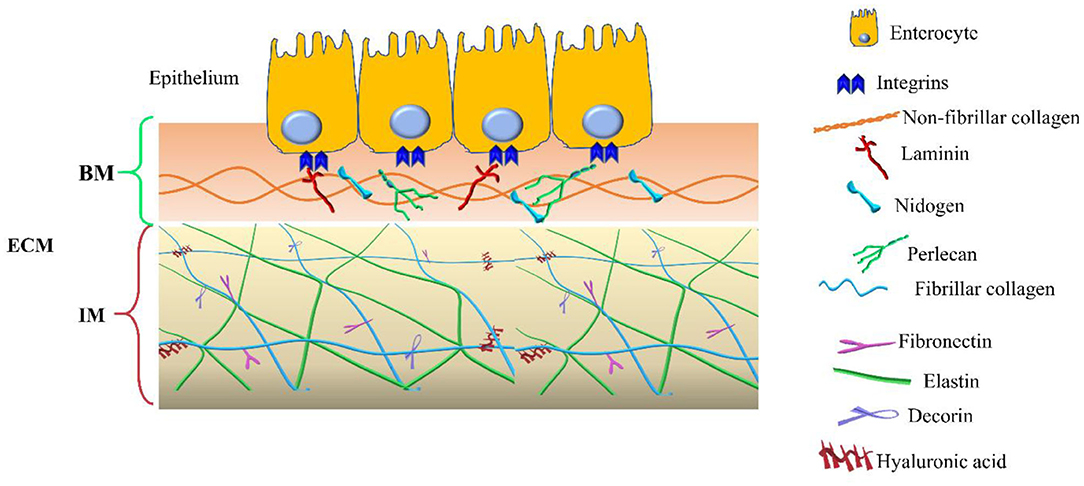
\includegraphics[width=15cm, height=7.5cm]{fmed-08-610189-g001}

\subsection{Technologies}

\begin{itemize}
    
    \item TRPS uses a tunable voltage, pore size and pressure to filter the particles in a more exact way adn detect their size and concentration. (-) Clotting of the pores is possible. (+) Measures the $\zeta$ potential at once. Which is related to the electrophoretic mobility.
    
    \item ExoView: technology that uses an antibody coated chip to capture EV's on the plate. After that stained antibodies detect the used antibody on these EV's. We could also use a mild detergent (SDS) to visualise the RNA molecules that are in the EV.
    (+) No complicated separation needed assessment is directly possible of the bio fluid. Immediately biological markers... (-) less quantitative (cost).
    
    \item Nano-FCM: low pressure sheath fluid and a reduced flow rate
    (+) estimation on the size, concentration also biological information. Multiple labels can be visualised at once. (-) The fluorescent technology needs to be applied in a fluid and so will also need to be removed again so there is no background signal during the cytometry step...
    
    \item AF4: First the smaller and then the larger particles will elude.
    here the labels wont need to be removed because these are very small particles and will so elude the first. (why do small particles elude first?! because these have a higher diffusion coefficient and will be able to get higher in the downwards applied stream and so be in the more center of the horizontal flow that is larger in the middle (parabolic pattern)) (+) The fluorescent particles don't need to be removed since these will elude first.
    
    \item EXODUS: Isolation technique. Exosome detection via ultra fast isolation system. Based on negative pressure oscillation and membrane vibration.
    
    \item Anion exchange chromatography: Uses the negative surface charge of EV's to select them (determined by the $\zeta$ potential)
    
    \item ELISA bead-base flow cytometry:
    ELISA or Enzyme-Linked Immunosorbent Assay is an immuno assay technique utilized to detect diseases. The principle of ELISA is antigen-antibody interaction.
    
    \item SDS-PAGE used to determine protein amount (see later)
    less polyacrylamide percentage (8\%, higher size pores) gives better resolution for heavier particles and higher percentage (12\%) for smaller kilo delton particles.
    It uses gelelectrophoresis: polyacrylamide gel. SDS binds non-covalent to the proteins and gives them a negative charge which is interesting with applying the electric field similar charge-to-mass ratio for all proteins. Smaller molecules travel faster. Higher MW higher negative charge
    
    \item PCR: utilises 3 steps: Denaturation (95°C), annealing (55°C), extension (72°C) followed by a 'Final Hold'

    The needed components are: DNA template, DNA polymerase, two primer (forward and reverse one and the primer design: the forward primer is complementary tot the 3' end of the anti-sense strand  and the reverse primer is complementary to the 3' end of the sense strand. the forward primer is the beginning of the gene and the reverse primer is is the reverrse compliment of the 3' end of the gene

    \item qPCR: monitors the amplification of DNa molecule during PCR and not at its end. done by using SYRB green fluorescences only when bound to double stranded DNA. Taqman probes has 2 parts (reporter and quencher) during PCR the probe is degraded and so releases the reporter. Certain fluorescence treshold correspond to relative level of gene expression

    \item Western Blotting
    \begin{itemize}
        \item Sample preparation: native or denatured proteins (sds?)
        \item Gel electrophoresis agarose (DNA or RNA) or polyacrylamude gel the appropiate gel concentration usage!
        \item membrane transfer
        \item Blocking: of all the non-occupied antibody binding sites on the membranes to prevent non-specific binding (albumine)
        \item Primary antibody incubation
        \item secondary antibody incubation
        \item detection
        \item Analysis
    \end{itemize}
    
    \item H\&E staining:
    Hematoxylin stains cell nuclei blue and Eosin stains cell cytoplasm and most connective tissue fibers in pink, orange and red.

    \item IHC: antibody-antigen detection you can also use multiple different stains to get overlaying colours. primary antibody that recognises the antigen (prefer monoclonal (mouse, rat) higher specificity) then use a secondary antibody to recognise this non human primary antibody and probe it with a (avidine-biotin complex to make it fluorescent) can be polyclonal (goat, rabbit) now cause only need to recognise not human. primary and secondary antibody should always come from different species.

    To reduce aspecifity you could put a coating on the cell that prohibits secondary antibody binding. After that apply the primary antibody that introduces now the only possible secondary antibody binding site :-)

    \item FISH: uses a labeled complementary DNA or RNA strand to localise a specific DNA or RNA sequence. Centromere probes, Single copy probes, Chromosome painting. First denaturate to add the probe of course! Also RISH very interesting to combine?!

\end{itemize}

\subsection{Cell culturing (general notes)}
Serum-free media presents an alternative to serum-containing media and offers several advantages, which include better understanding of media composition, reduced cost, and a reduced risk of contamination by infectious agents found in serum

37°C + 5\% CO2

cadherins (cell-cell adhesion)(Na2+)
integrins( cell-ECM adhesion)

3 steps in sub culturing:
\begin{itemize}
    \item cell collection
    \item cell counting
    \item cell seeding
\end{itemize}
PH is maintained using a buffer system. Mycoplasms contamination is not visible

cell cultures could be used in: basic research, Bio pharmaceutical manufacturing, Bio compatibility and drug testing personalised systems, Cell-based therapies and Tissue engineering, 

But also limitations: a cell culture really doesn't simulate real body environment. E.g.: 2d situations (which are stiff resistance to deformation etc), most of the time only 1 cell type at the time. cell lines have been cultured for multiple generations resulting into a drift of their characteristics.
But also limitations due to the culture conditions. Lack of co-culture models see slide 33!!!

Cellular senescence: irreversible growth arrest

\subsection{Quantitative assays to measure cellular contents and activities}

\begin{itemize}
    \item End-point assays
    \begin{itemize}
        \item Metabolic activity (MTT)
        \item Dye exclusion assays
        \item ATP assays
        \item Protein content, DNA/RNA content
        \item Image-based microscopy
    \end{itemize}
    \item Longitudinal assays
    \begin{itemize}
        \item Impedance based(xCelligence
        \item Image based(Cell imaging videomicroscopy
        \item (IncuCyte)
    \end{itemize}
\end{itemize}

Phenotypic assays:
\begin{itemize}
    \item metabolic activity: MTT
    \item DNA synthesis using Bromodeoxyuridine (BrdU) can be recognised with antibodies
    \item membrane markers (trypan blue, or calcein-AM(live) + propidiumiodide (dead))
    \item protein content (SRB Sulphorhodamine B)  
    \item protein content: SDS-PAGE
    
    
    Followed by:
    \begin{itemize}
        \item Western blot analysis: used antigen-antibody interaction using a membrane transfer to another gel
        \item Commassie blue staining: dye interacts electrostatically
        \item Silver staining for (specific) protein detection: more specific 100x
    \end{itemize}
    \item longitudinal assays 
    \begin{itemize}
        \item growth (use less cells in a well to have a longer growth curve) wells with more cells can be used to better study cell death since these have less steep death curves that happen not that long after the start of the assay
        \item migration (transwell migration, chemoattractant at the bottom)
        \item invasion (in the transwell now there is a matrigel layer added
    \end{itemize}
\end{itemize}

In general it is always use-full to end a longitudinal assay with an end-point one so you don't waste possible to acquire information.

\subsection{Tissues (general notes)}
Main Tissue types:
\begin{itemize}
    \item Epithelial Tissue
    
    \item Connective Tissue
    
    \item Muscle Tissue
    
    \item Nervous Tissue
    
\end{itemize}
Know their characteristics
\subsection{Tissue Analysis}

Important steps!:
\begin{itemize}
    \item Sampling: Ischemia (restriction of the blood supply) degrades the tissue
    \item Fixation: aim is to preserve the tissue in the least altered situation in regard to the in vivo state possible. IMO the most important step in this whole process because this will determine the tissues characteristics the most in the later stadia.
    \item Dehydration
    \item Clearing
    \item Impregnation
    \item Sectioning
    \item Staining
    \item Dehydration
    \item Clearing
    \item Mounting
\end{itemize}

IHC: Avidine-biotine complex! Avidin can bind up to 4 fluorophores

\subsection{Tissue/Tumor engineering}
Typical process of tissue engineering
\begin{itemize}
    \item Imaging and design (CT and MRI)\\
    Computed topography: based on the variable tissue absorption of X-rays
    X ray source rotates around the body and sensors measure the transmitted beam intensity and angle\\
    
    Magnetic resonance imaging: uses nuclear magnetic resonance: strong magnetic field causes a small fraction of the nuclei in the tissue to align themselves with the magnetic field. Contrast agents can be used too greatly increase the contrast.
    \item Choice of material and cells (synthetic or natural polymers and decellullarised ECM)
    Advantage of natural polymers is their similarity to the human ECM and their inherent bio-activity. Advantage of synthetic polymers is that they can be tailored with specific physical properties\\

    Material properties for bio-printing:
    \begin{itemize}
        \item Printability: viscosity not to high, enough cross-linking
        \item Bio-compatibility: an active and controllable contribution to the biological and functional components of the construct
        \item Degradation kinetics: ability to control the degradation rates, ideally matching with the ability of the ells to replace the materials with their own ECM. degradation products should not be toxic.
        \item Structural and mechanical properties
        \item material biomimicry
    \end{itemize}
    \item Printing of the tissue construct
    \item Application
\end{itemize}

Design approaches
\begin{itemize}
    \item Biomimicry: is a technique in which the bio printer creates structures that mimic the natural structures found in living organisms. For example, a bio printer could create a 3D model of a blood vessel or a bone by replicating the structure and composition of these tissues in the body.
    \item Autonomous self-assembly: This approach involves the use of bioinks and other materials that are designed to self-assemble into a specific 3D structure. The bioprinter creates a template or scaffold for the materials to build upon, and the materials themselves are programmed to spontaneously arrange themselves into the desired 3D structure. (starts from stem cells whereas biomimicry started from allready selected cell types!)
    \item Mini tissue building blocks: This approach involves creating small, standardized units or "building blocks" of tissue, which can then be assembled into larger structures. The bio printer places these building blocks in a specific pattern to create the desired 3D structure. This approach allows for the creation of more complex structures, such as organs or organoids, by combining multiple building blocks.(nephrons)\\
    There are 2 main strategies for this: self-assembling cell spheres and accurate, high resolution reproductions of a tissue unit
\end{itemize}

Decellularised scaffolds produced by perfusing organs with detergents that remove all cellular and immunogenic species. cells + ECM completely removed, only keep the shapes.

matrigel: main component is laminin so it resembles the basement membrane

Cell sources: endogenous stem cells, autologous source of cells. Stemm cells are interesting because of their multipotent state but undifferentiated reproduction. Also induced pluripotent cells exist\\

Tissue bioprinting strategies:(know the cons and pros)
\begin{itemize}
    \item Inkjet bioprinting; Thermal or Piezoelectric
    \item Micro-extrusion bioprinting
    \item laser-assited bioprinting
\end{itemize}

Organoids: self-organisation, Multicellularity, functionality. Could be used because they resemble the tissue sometimes very good. Could predic respond on treatments of patients without having them go through intense treatments\\

A patient-derived xenograft (PDX) is a type of animal model that is used in research and drug development. It is created by transplanting a piece of cancer tissue from a patient into an immunodeficient animal, such as a mouse or rat. The cancer tissue is able to grow and form a tumor in the animal, which is similar to the original tumor in the patient. PDX models are used to study the biology of cancer and to test the effectiveness of new treatments.\\

Organ-on-chip: can easily recreate cell-ECM or cell-cell interactions they solve the 3d troubles of in vitro models. microfluid models of metastasis
\pagebreak
\section{Exam questions}
Remember that these are generated using AI so it may be to deeply detailed or missing some essential details from in the lesson. These results are purely to give you a little background localisation in the booklets.

A fluorescence molecule, also known as a fluorophore, is a molecule that is able to absorb light energy at a specific wavelength and then re-emit that energy at a different wavelength. In order for a molecule to be able to exhibit fluorescence, it must have certain characteristics:
\begin{itemize}


\item The molecule must have a structure that allows it to absorb light energy at a specific wavelength. This typically involves the presence of a conjugated system of double bonds, which can absorb light in the visible or ultraviolet (UV) range.

\item The molecule must also have a way to release the absorbed energy, typically through the emission of a photon of light. This is usually achieved through the presence of a suitable chemical group or functional group, such as a phenyl ring or a nitrogen-containing group.

\item The molecule must also have a relatively high quantum yield, which refers to the fraction of absorbed photons that are converted into emitted photons. If the quantum yield is too low, the fluorescence signal will be weak and difficult to detect.

\item The molecule should also have a suitable fluorescence lifetime, which is the amount of time it takes for the molecule to relax back to its ground state after emitting a photon of light. If the lifetime is too long, the fluorescence signal will be weak and difficult to detect. On the other hand, if the lifetime is too short, the fluorescence signal will be difficult to distinguish from background fluorescence or other sources of light.
\end{itemize}

Overall, a fluorescence molecule should have a suitable absorption spectrum, a suitable emission spectrum, a relatively low quantum yield, and a suitable fluorescence lifetime in order to be able to exhibit fluorescence effectively.

Some AI generated answers to the VTK wiki document because i did not want to type a lot...

AFM (Atomic Force Microscopy) is a technique used to visualize and manipulate samples at the nanoscale. It works by using a very fine probe, or tip, to scan the surface of a sample and measure the forces between the tip and the sample. There are several different modes of AFM, including contact mode, non-contact mode, and lateral force mode.\\

Forces are interactions that cause objects to accelerate or decelerate. They can be attractive or repulsive, and can be caused by a variety of physical phenomena, such as gravity, electromagnetism, and the strong and weak nuclear forces.\\

Animal cells and plant cells are both types of eukaryotic cells, meaning they have a defined nucleus and other membrane-bound organelles. However, there are some key differences between the two types of cells. Plant cells have a cell wall, chloroplasts, and large central vacuoles, while animal cells do not. Mitochondria are organelles found in most eukaryotic cells that are responsible for producing energy for the cell through the process of cellular respiration. Lysosomes are organelles that contain enzymes that break down waste materials and cellular debris. Peroxisomes are similar to lysosomes, but they contain enzymes that specifically break down peroxides and other toxic substances.\\

An enzyme is a protein that catalyzes chemical reactions in the body. The Michaelis-Menten equation is a mathematical equation used to describe the rate of an enzymatic reaction as a function of the substrate concentration. The equation can be linearized by performing a double reciprocal plot, also known as a Lineweaver-Burk plot. Competitive inhibitors are molecules that bind to the same site on the enzyme as the substrate, preventing the substrate from binding and inhibiting the enzyme's activity. Non-competitive inhibitors bind to a different site on the enzyme, altering the enzyme's conformation and inhibiting its activity. Uncompetitive inhibitors bind to the enzyme-substrate complex and inhibit the enzyme's activity.\\

DIC (Differential Interference Contrast) microscopy is a technique used to visualize samples that are otherwise difficult to see due to low contrast or lack of intrinsic fluorescence. It works by using two beams of light that are slightly out of phase with each other to produce a contrast-enhancing interference pattern. Phase contrast microscopy is a similar technique that uses a special objective lens and a phase plate to produce a contrast-enhancing interference pattern.\\

One way to improve the resolution of an imaging program is to use deconvolution algorithms, which can mathematically "unblur" the image and improve the resolution. Another option is to use superresolution techniques, such as STED (Stimulated Emission Depletion) microscopy, which can achieve resolutions beyond the diffraction limit of traditional light microscopes.\\

STED microscopy works by using a laser beam to selectively deplete the fluorescence of certain areas of the sample, creating a "dark" region that can be used to define the resolution of the image. This is achieved by using a second laser beam to stimulate the emission of fluorescence from the sample, and then using a depletion beam to cancel out the fluorescence in a specific region. STED microscopy has a variety of applications, including imaging of living cells and tissues, and imaging of protein-protein interactions.\\

The critical angle of total internal reflection is the angle of incidence at which light will be completely reflected at the interface between two media with different refractive indices. It is determined by the relationship between the refractive indices of the two media, and can be calculated using the formula:

critical angle = $arcsin(n2/n1)$
where n1 and n2 are the refractive indices of the two media.

The intensity of the reflected light decreases with distance from the substrate due to losses due to absorption and scattering.\\

A fluorescent molecule must have the ability to absorb light of a specific wavelength and re-emit light at a longer wavelength. This process is known as fluorescence, and it is what gives fluorescent molecules their distinctive bright colors. Fluorescent molecules also typically have a high quantum yield, meaning they are efficient at converting absorbed light into fluorescence.\\

Flow cytometry is a technique used to analyze and sort cells based on their physical and biochemical properties. It works by passing cells through a flow cytometer, which uses lasers and detectors to measure the characteristics of the cells as they pass through. The flow cytometer can be used to analyze cells in terms of size, granularity, and fluorescence, and it can sort cells based on these characteristics. Flow cytometry has a variety of applications, including cell counting, cell sorting, and analysis of protein expression.\\

Fluorescence correlation spectroscopy (FCS) is a technique used to measure the dynamics of fluorescent molecules in solution. It works by using a laser to excite the fluorescent molecules and a detector to measure the fluorescence intensity as a function of time. By analyzing the fluctuations in fluorescence intensity, FCS can provide information about the diffusion, concentration, and interactions of fluorescent molecules in solution. FCS has a variety of applications, including the study of protein-protein interactions, protein folding, and gene expression.\\

The efficiency of FRET (Förster Resonance Energy Transfer) is a measure of how efficiently energy is transferred between two fluorescent molecules that are in close proximity to each other. The efficiency of FRET depends on the distance between the two molecules, as well as the Forster radius, which is a measure of the distance at which the efficiency of FRET begins to decline. If the distance between the two molecules is 1.5 nm and the Forster radius is 3 nm, the efficiency of FRET will be high. If the distance between the molecules is 6 nm and the Forster radius is 3 nm, the efficiency of FRET will be lower. If the Forster radius is 6 nm, the efficiency of FRET will be even lower, regardless of the distance between the molecules.\\

Samples for SEM (Scanning Electron Microscopy) need to be dried and coated with a thin layer of a conductive material, such as gold or platinum, to prevent charging during the imaging process. TEM (Transmission Electron Microscopy) samples need to be thinned to a thickness of less than 100 nm, typically using a combination of mechanical and chemical techniques.\\

Mass spectrometry is a technique used to identify and quantify the components of a sample based on their mass-to-charge ratio. It works by ionizing the sample and measuring the masses of the resulting ions using a mass spectrometer. The mass spectrometer works by accelerating the ions through an electric field and then measuring their motion through a magnetic field. The motion of the ions is affected by their mass-to-charge ratio, so by measuring the motion of the ions, it is possible to determine their mass. Mass spectrometry has a variety of applications, including the identification and quantification of small molecules, proteins, and other biomolecules, and the analysis of complex mixtures.\\

Liquid chromatography is a technique used to separate and purify samples based on their interactions with a stationary phase and a mobile phase. It works by passing a sample through a column filled with the stationary phase, and then measuring the movement of the sample as it interacts with the stationary phase. The stationary phase can be a solid, such as silica or alumina, or a liquid, such as a polymer. The mobile phase can be a gas or a liquid. The separation of the sample is based on the interactions between the stationary phase and the sample, and the movement of the sample through the column is determined by the properties of the mobile phase. Liquid chromatography has a variety of applications, including the purification of small molecules, proteins, and other biomolecules, and the analysis of complex mixtures.\\

Last questions are literally fill in the formula for reduced mass and remember how the unit 1/cm works (wave number == frequency/c)



\begin{itemize}
    \item Question 1:
    
There are four main types of tissue in the body: epithelial tissue, connective tissue, muscle tissue, and nervous tissue.\\

Epithelial tissue is a type of tissue that covers the surface of the body and lines body cavities and organs. It is made up of cells that are closely packed together and are supported by a basement membrane. Epithelial tissue has three main characteristics:\\
\begin{itemize}
\item Polarity: Epithelial cells have an apical surface, which faces outward or away from the body, and a basal surface, which faces inward or towards the body.

\item Avascularity: Epithelial tissue has no blood vessels and relies on diffusion to obtain nutrients and remove waste.

\item Regeneration: Epithelial tissue has a high capacity for regeneration, meaning it can quickly repair itself after damage.
\end{itemize}
Connective tissue is a type of tissue that provides support and protection to the body. It is made up of cells that are widely spaced and are embedded in a matrix of extracellular material. Connective tissue has three main characteristics:\\
\begin{itemize}
\item Diversity: Connective tissue comes in many different types, including bone, cartilage, and blood, each of which has its own unique characteristics.

\item Specialized cells: Connective tissue contains a variety of specialized cells, including fibroblasts, macrophages, and leukocytes, which perform specific functions.

\item Matrix: Connective tissue has a matrix that is composed of extracellular material, such as collagen, elastin, and ground substance, which gives it its structural and functional properties.
\end{itemize}
Muscle tissue is a type of tissue that is responsible for movement and the generation of force. It is made up of cells that are specialized for contraction and relaxation. Muscle tissue has three main characteristics:\\
\begin{itemize}
\item Contractility: Muscle cells are able to contract and relax in response to stimuli, allowing them to generate force and movement.

\item Excitability: Muscle cells are able to respond to stimuli such as electrical signals, allowing them to be controlled by the nervous system.

\item Extensibility: Muscle cells are able to stretch and elongate when contracting, allowing them to generate large amounts of force over a wide range of motion.
\end{itemize}
Nervous tissue is a type of tissue that is responsible for the transmission of electrical signals throughout the body. It is made up of cells called neurons and glial cells. Nervous tissue has three main characteristics:\\
\begin{itemize}
\item Conductivity: Nervous tissue is able to conduct electrical signals, called action potentials, from one part of the body to another.

\item Excitability: Nervous tissue is able to respond to stimuli, such as changes in the environment or the activity of other cells, by generating and transmitting action potentials.

\item Integration: Nervous tissue is able to integrate and process information from various sources, allowing it to coordinate and control the functions of the body.
\end{itemize}
The cells shown in the image are called endothelial cells, and they have a squamous shape, meaning they are flat and scale-like. The cells are arranged in a single layer, with their nuclei located near the center of the cells. The staining technique used in the image is H\&E (Hematoxylin and Eosin), which is a commonly used histological staining technique that is used to visualize the structure of tissues. Hematoxylin is a basic dye that stains nuclei and other cellular\\

Hematoxylin staining: Hematoxylin is a basic (alkaline) dye that is used to stain the nucleus of cells blue. It binds to the DNA and RNA in the nucleus, making it visible under the microscope. The tissue is first treated with a mordant, which helps the hematoxylin to bind to the tissue. The tissue is then soaked in a solution of hematoxylin, which is absorbed by the cells.

Eosin staining: Eosin is an acidic dye that is used to stain the cytoplasm and other intracellular structures pink. It binds to proteins and other cellular components, making them visible under the microscope. After the tissue has been stained with hematoxylin, it is treated with a solution of eosin, which is absorbed by the cells.

    \item Question 2:
Polymerase chain reaction (PCR) is a laboratory technique that is used to amplify small amounts of DNA. It is an essential tool in molecular biology and is widely used in medical, forensic, and research laboratories.\\

The steps involved in PCR are:
\begin{itemize}
\item Denaturation: The DNA template is heated to a high temperature to separate the two strands of the double helix.

\item Annealing: The temperature is lowered to allow primers (short DNA sequences) to bind to specific locations on the template DNA. The primers are used to mark the beginning and end of the region of DNA that is to be amplified.

\item Extension: The temperature is raised again to allow a heat-stable enzyme called a polymerase to extend the primers by adding new nucleotides (the building blocks of DNA) to the ends. This creates new DNA strands that are complementary to the template strands.
\item Repeat: The process is repeated multiple times, typically between 20 and 40 cycles. Each cycle doubles the amount of amplified DNA.
\end{itemize}

To perform PCR, you need the following components:
\begin{itemize}
\item DNA template: This is the small amount of DNA that you want to amplify.
\item Primers: These are short DNA sequences that are complementary to specific regions of the template DNA.

\item Nucleotides: These are the building blocks of DNA and are used by the polymerase to synthesize the new DNA strands.

\item Polymerase: This is the enzyme that synthesizes the new DNA strands by adding nucleotides to the ends of the primers.

\item Buffer: This is a solution that contains all the necessary components for PCR, such as salts, enzymes, and cofactors.
\end{itemize}

One assay that studies the same cellular content as PCR is real-time PCR (also known as quantitative PCR or qPCR). This technique is similar to PCR, but it includes an additional step in which the amplified DNA is measured as it is being produced. This allows researchers to determine the amount of DNA present at each cycle of the reaction, providing a more accurate and sensitive measurement of the DNA template.
    \item Question 3:
Migration and invasion are two processes that can occur in cells during tissue remodeling or cancer progression.\\

Migration refers to the movement of cells from one location to another within a tissue. This process is important for the repair and healing of tissues, as well as for the development and maintenance of normal tissue architecture.\\

Invasion refers to the ability of cells to penetrate and migrate through the extracellular matrix (ECM) and into surrounding tissues. This process is important in cancer, as cancer cells can invade and spread to other parts of the body, leading to metastasis.\\

Matrigel and collagen are two types of ECM proteins that are commonly used in cell culture experiments.\\

Matrigel is a protein mixture that is derived from the Engelbreth-Holm-Swarm (EHS) mouse sarcoma. It contains a variety of ECM components, including laminin, collagen, and glycosaminoglycans. Matrigel is commonly used to study cell migration, invasion, and differentiation, as it provides a three-dimensional matrix that more closely resembles the natural ECM found in tissues.\\

Collagen is a protein that is abundant in the ECM of many tissues, including skin, bone, and blood vessels. It is a major component of the ECM and is important for the structural integrity and mechanical strength of tissues. Collagen is commonly used to study cell adhesion, migration, and differentiation, as well as tissue engineering.\\

Longitudinal assays are experiments that are conducted over a period of time, with measurements taken at multiple time points. These types of assays are useful for studying processes that occur over time, such as cell growth, differentiation, or disease progression.\\

End-point assays are experiments that are conducted for a fixed period of time, with a single measurement taken at the end of the experiment. These types of assays are useful for studying the final outcome or endpoint of a process, such as cell survival, proliferation, or gene expression.\\

It is important to do both longitudinal and end-point assays because different types of experiments are suitable for different research questions. For example, if you are studying the progression of a disease over time, a longitudinal assay would be more appropriate, as it would allow you to track changes in the disease state over time. However, if you are studying the effect of a particular treatment on the survival of cells, an end-point assay would be more suitable, as it would allow you to determine the final outcome of the treatment.\\

An example of a study where both longitudinal and end-point assays are done is a clinical trial to evaluate the effectiveness of a new drug for treating cancer. In this study, patients would be followed over time to track the progression of their cancer and the effectiveness of the drug. End-point measurements, such as survival rate or response rate, would be taken at the end of the trial to determine the overall effectiveness of the drug. Longitudinal measurements, such as tumor size or quality of life, would be taken at multiple time points throughout the trial to track the changes in the cancer state over time.\\

    \item Question 4:

One type of bioprinter that could be used for this purpose is a inkjet bioprinter. Inkjet bioprinters use a nozzle to deposit small droplets of cells or biomaterials onto a substrate, allowing for precise control over the placement and orientation of the cells. Inkjet bioprinters are suitable for printing cells with high viability, as the cells are not subjected to high shear forces or extreme temperatures during the printing process.\\

Another type of bioprinter that could be used is a laser-assisted bioprinter. Laser-assisted bioprinters use a focused laser beam to manipulate cells or biomaterials, allowing for precise control over the position and orientation of the cells. Laser-assisted bioprinters are suitable for printing cells with high viability, as the cells are not subjected to high shear forces or extreme temperatures during the printing process.

Trypan blue assay

    \item Question 5:

Try to solve using FISH\\

Yes, fluorescence in situ hybridization (FISH) can be used to detect the presence of two different genes in the same tissue sample. FISH is a laboratory technique that involves applying labeled probes to a tissue sample and examining the sample under a microscope to detect the presence and location of the probes within the tissue. The probes are typically labeled with a fluorescent dye or a radioactive isotope, and are specific for the genes of interest.\\

To detect the presence of two different genes in the same tissue sample using FISH, you would need to design and synthesize two probes, one for each of the genes. The probes would be labeled with different fluorescent dyes or isotopes, so that they can be distinguished from each other when viewed under a microscope. The probes would then be applied to the tissue sample and allowed to hybridize (bind) to the target genes.\\

The most crucial step in the process of sectioning and staining tissue samples for microscopy is the fixation step. Fixation is the process of preserving the tissue samples by chemically crosslinking the proteins and other biomolecules in the tissue. Fixation is important because it helps to preserve the tissue structure and prevent degradation, allowing the tissue to be sectioned and stained for microscopy without falling apart. Fixation is typically achieved using a chemical fixative, such as formalin or ethanol. The choice of fixative and the fixation protocol will depend on the specific requirements of the experiment and the type of tissue being studied.
    
\end{itemize}

\end{document}


